\chapter{Computation}

\subsection{Complexity}

Big-O notation is typically used to approximate the time dependence on the number of elements you feed into an algorithm. In Big-O notation, we ignore all lower order terms, and also forget about any leading constants.

Listed are some standard algorithms and their dependence.

\begin{center}
\begin{tabular}{ | c | c|} 
\hline
 $N$-Dependence & Algorithm\\ \hline
$O(1)$ & Accessing an element in an array  \\ 
$O(\log N)$ & Binary Search  \\
$O(N)$ & Single \texttt{for} loop \\ 
$O(N^2)$ & Simple sorting algorithm (bubble, selection, ...)\\
$O(c^N)$ & Solving the travelling salesman problem with dynamic programming \\
$O(N!)$ & Iterations over all combinatorics \\
\hline
\end{tabular}
\end{center}

\subsection{Efficient Algorithms}

\subsection{Averaging}
When updating an average which contains many elements, the naive way of calculating the average is $O(n)$ efficient 
\begin{align}
	\langle x_{n-1}\rangle = \frac{1}{n-1}\sum_{i=0}^{n-1} x_i
\end{align}
When constantly updating the average, we can use the following equivalent formula
\begin{align}
	\langle x_{n}\rangle &= \frac{1}{n}\sum_{i=0}^{n} x_i\\
	&= \frac{1}{n}\Big(x_n + (n-1)\langle x_{n-1}\rangle\Big)\\
	&= \langle x_{n-1}\rangle + \frac{1}{n}\Big(x_n - \langle x_{n-1} \rangle\Big)
\end{align}
This modified algorithm is $O(1)$ efficient.

\subsection{Estimating Probabilities}
When multiplying many different probabilities $p_i$ together, the floating point precision of many computing languages starts to become an issue. To avoid this problem, often $\log(p_i)$ is used which is monotonic with the probability but avoids the \textit{underflow} issue described.

\subsection{Graph Theory}
Brute force algorithms that search all combinations of $N$ items scale as $N!$. The Seven Bridges of Konigsberg is a famous example solved by Euler, for which he laid our all combinations of sequences you could possibly cross the seven bridges (e.g. $1234567, 1234576,...$ and was able to show each combination did not work.

\subsection{Bin Error}
A histogram bin can be treated using Poisson statistics, which makes it's error $\sqrt{n}$ where $n$ is the number of entries in the bin.

\section{Regression}
\subsection{Linear Regression}\label{least-squares}
Let's pretend we are fitting a straight line, so we have a bunch of independent variables $x_i$ and their corresponding measured values $y_i$. We pick for our model

\begin{align}
y_i = ax_i + b
\end{align}

Now the thing we want to do is minimize $\chi^2$ for the full combination of points. We do this of course, by taking a derivative to find the minimum. For simple illustrative purposes, lets take $\sigma_i$, the measurement error, to be the same for each point. For $a$ we have
\begin{align}
\frac{\partial \chi^2}{\partial a} = 0 &= \frac{\partial}{\partial a} \sum_i \frac{\Big(y_i - (ax_i + b)\Big)^2}{\sigma_i^2} \\
&= - \frac{2}{\sigma^2}\sum_i \Big(y_i - (ax_i+b)\Big)x_i\\
&= \sum_i y_i x_i - a\sum_ix_i^2 - b\sum_i x_i
\end{align}
Similarly, for $b$
\begin{align}
\frac{\partial \chi^2}{\partial b} = 0 &= -\frac{2}{\sigma^2}\sum_i \Big(y_i-(ax_i+b)\Big)\\
&= \sum_i y_i - a \sum_i x_i - b
\end{align}
Now we have a set of linear equations. We can easily calculate all of the sums, since they are by definition the data we are fitting to, and after some algebra, we can solve for the $a$ and $b$ which minimize $\chi^2$.
\begin{align}
b &= \sum_i y_i - a \sum_i x_i\\
\rightarrow 0 &= \sum_i y_i x_i - a\sum_ix_i^2 - \Big(\sum_i y_i - a \sum_i x_i\Big)\sum_i x_i\\
\sum_i y_i x_i  - \sum_j y_j \sum_i x_i &= a\Big[\sum_i x_i^2 -\Big(\sum_i x_i\Big)^2\Big]\\
a &= \Big[\sum_i y_i x_i  - \sum_j y_j \sum_i x_i\Big] /\Big[\sum_i x_i^2 -\Big(\sum_i x_i\Big)^2\Big] 
\end{align}
In a computer program, it would look like


\lstinputlisting[language=Python]{mathematics/code/linearRegression.py}


\centering{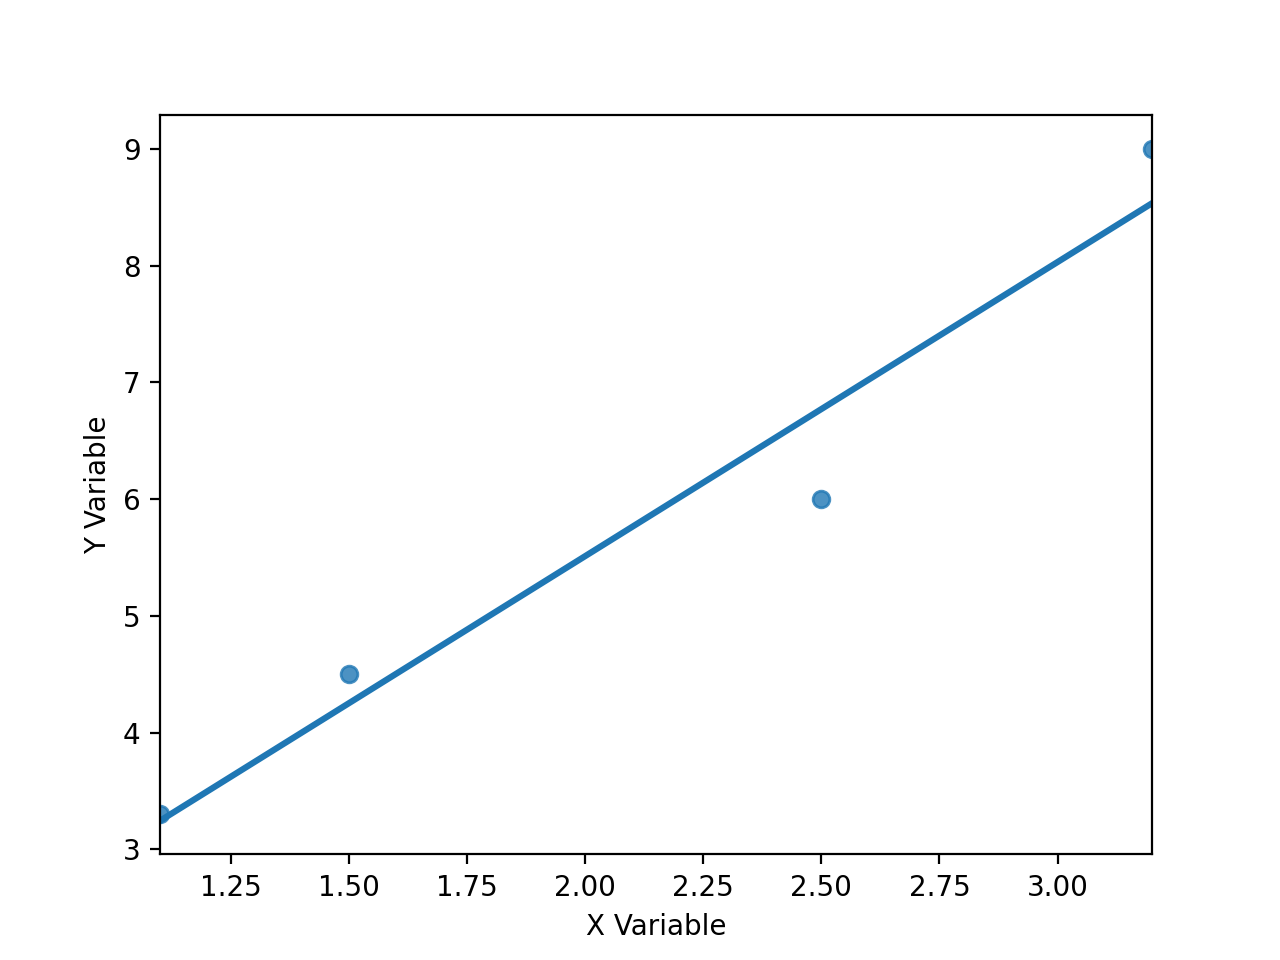
\includegraphics[width=0.5\textwidth]{mathematics/fig/linearRegression.png}}


\subsection{Multiple Regression}
Multiple regression is just linear regression done for more than one feature dimension. In general the problem it solves is of the form
\begin{align}
	\min_w||Xw-y||^2_2
\end{align}
Where $w$ is the weight vector, $x$ is the feature vector (including a term for the intercept) and $y$ is the label.

\subsection{Ridge Regression}
Ridge regression is a linear regression with an added penalty term proportional to the sum of the squared weights. This effectively prevents the model from becoming heavily dependent on a single weight and therefore is helpful in situations where the feature vectors are correlated (multicollinearity). The function to minimize is 
\begin{align}
	\min_w||Xw-y||^2_2 + \alpha||w||^2_2
\end{align}

\subsection{Lasso}
The LASSO (Least Absolute Shrinkage and Selection Operator) is designed to minimize the number of features the model is dependent on. The function it minimizes is 

\begin{align}
	\min_w\frac{1}{2n_{\textrm{samples}}}||Xw-y||^2_2 + \alpha||w||_1
\end{align}

Lasso can set weights to 0, while Ridge regression cannot.


